 \begin{center}\begin{large} Final Test
 \vspace{1em}
 
 \end{large}\end{center}
 \small Each question is worth one point. Duration: 150 minutes.
 \bigskip

 
\begin{problem}
Find the value of the expression:
\[ (3\va+4\vb)\cdot (\va-2\vc), \]
where $\va=[2, 3, 2]^T,\,\vb=[0, -3, 2]^T,\,\vc=[-2, 5, -1]^T$.
\end{problem}
\medskip

\begin{problem}
Calculate the L1 (Manhattan) and L2 (Euclidean) norms of the following vector:
\[ \dfrac{1}{3}\va+\dfrac{2}{3}\vb, \]
where $\va=[-5,4,10]^T,\,\vb=[1,0,7]^T$.
\end{problem}
\medskip

\begin{problem}
Find the angle between $\va$ and $\vb$ in the previous problem.
\end{problem}
\medskip

\begin{problem}
Find the dimension of $\operatorname{span}\{\vv_1,\vv_2,\vv_3\}$ if
\[
\vv_1 = \begin{bmatrix}
    7 \\ 2 \\ 5
\end{bmatrix},
\qquad
\vv_2 = \begin{bmatrix}
    4 \\ 4 \\ 14
\end{bmatrix},
\qquad
\vv_3 = \begin{bmatrix}
    -11 \\ 4 \\ 20
\end{bmatrix}.
\]
\end{problem}
\medskip

\begin{problem}
Given the matrices
\[ A = \begin{bmatrix}
-1&0&0&-2\\1&0&5&-5\\0&1&4&0\\0&0&-5&0
\end{bmatrix},\qquad B = \begin{bmatrix}
4&3&4&2\\8&7&5&3\\4&3&8&5\\4&3&4&3
\end{bmatrix}, \]
find $\det(AB)$.
\end{problem}
\medskip

\begin{problem}
Solve the SLE:
\[
\begin{cases}
    4x - y + 3z = 2\\
    11x + 4y - 9z = 11\\
    x + 2y - 5z = 3
\end{cases}
 \]
\end{problem}
\medskip


\begin{problem}
Check if the matrix is positive definite:
\[ A = \begin{bmatrix}
2& -1& 0& 3\\
-1& 2 &-1 & 2\\
0& -1& 2 & 1 \\
-4& -2& -4 & 3 
\end{bmatrix}.\]
\end{problem}
\medskip

\begin{problem}
Find the algebraic and geometric multiplicities of the eigenvalues of the following matrix:
\[ A = \begin{bmatrix}
7 &0& -3\\
-9 &-2& 3\\
18 &0& -8

\end{bmatrix}. \]
\end{problem}
\medskip


\begin{problem}
Find the points of local extrema of the following function:
\[ f(x) = x^{2}+\ln\left(x+3\right), \]
and check if they are minimum or maximum points.
\end{problem}
\medskip



\begin{problem}
Find the area under the graph of the following function between the lines $x=0$ and $x=2$:
\[ f(x) = x^{2}+\frac{\sin\left(\pi x\right)}{\pi} \]
\end{problem}
\medskip



\begin{problem}
Compute the gradient of the function:
\[ f(x,y,z) = \dfrac{3x^2e^{1-z^2}}{y} \]
at the point $(-2,3,1)$.
\end{problem}
\medskip



\begin{problem}
Compute the directional derivative of the function:
\[ f(x,y) = x^2 + 2xy - y^2 \]
in the direction of $[0.6,\;0.8]^T$ at the point $(1, 1)$.
\end{problem}
\medskip

\begin{problem}
Find the points of local extrema of the following function:
\[f(x, y) = x^4 - 4x^2 + y^2\]
Check if they are minimum or maximum points.
\end{problem}
\medskip



\begin{problem}
Two fair dice are rolled. What is the probability of getting $4$ on exactly one of them, given that their sum is even?
\end{problem}
\medskip


\begin{problem}
There are $8$ books on a bookshelf, $3$ on culinary, $5$ on arts. Hakob randomly takes three of them. What is the probability that all of those three are on the same subject?
\end{problem}
\medskip

\begin{problem}
The first album contains twice as much songs than the second. Moreover, $20\%$ of songs in the first album are in Armenian, while in the second album $45\%$ are. The DJ plays a random song in Armenian. What is the probability that the song was from the first album?
\end{problem}
\medskip


\begin{problem}
We toss a coin, and if it's heads we win \$2. Otherwise, we toss it once more, and if it's heads we win \$1, if it's tails, we win \$3. What is the probability of winning more than \$1 in this game?
\end{problem}
\medskip



\begin{problem}
Anna and Ani plan to meet each other somewhere between 19:00 and 20:00. If Ani arrives sooner than Anna, she waits for another $10$ minutes, and if Anna doesn't come, she leaves. If Anna arrives sooner than Ani, she waits for $5$ minutes, and if Ani doesn't come, she leaves. What is the probability that they will meet if both of them arrive at some random time between 19:00 and 20:00?
\end{problem}
\medskip

\begin{problem}
\\~\\
\begin{center}
    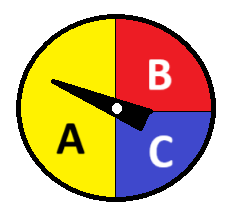
\includegraphics[width=0.2\linewidth]{figs/spinner.png}
\end{center}
\\~\\
You spin the spinner depicted above, and if it lands in the zone A, you win \$14; if it lands in the zone B, you win \$3; and if it lands in the zone C, you lose \$10. What is the expected amount of money you will win? 
\end{problem}
\medskip


\begin{problem}
Let $X$ be a random variable with the following PDF:
\[
f_X(x) = \begin{cases}
    (x-1)^3, & 1 \le x \le 3 \\
    0, & \text{otherwise}
\end{cases}
\]
Find the expectation and variance of $X$. 
\end{problem}

